\documentclass{article}
\usepackage[utf8]{inputenc}
\usepackage{graphicx}

\title{CSCM37 coursework 1}
\author{David Saunders (910995)}
\date{February 2020}

\begin{document}
\maketitle

\section*{Part 1, design 1}

\begin{figure}[ht]
\centering
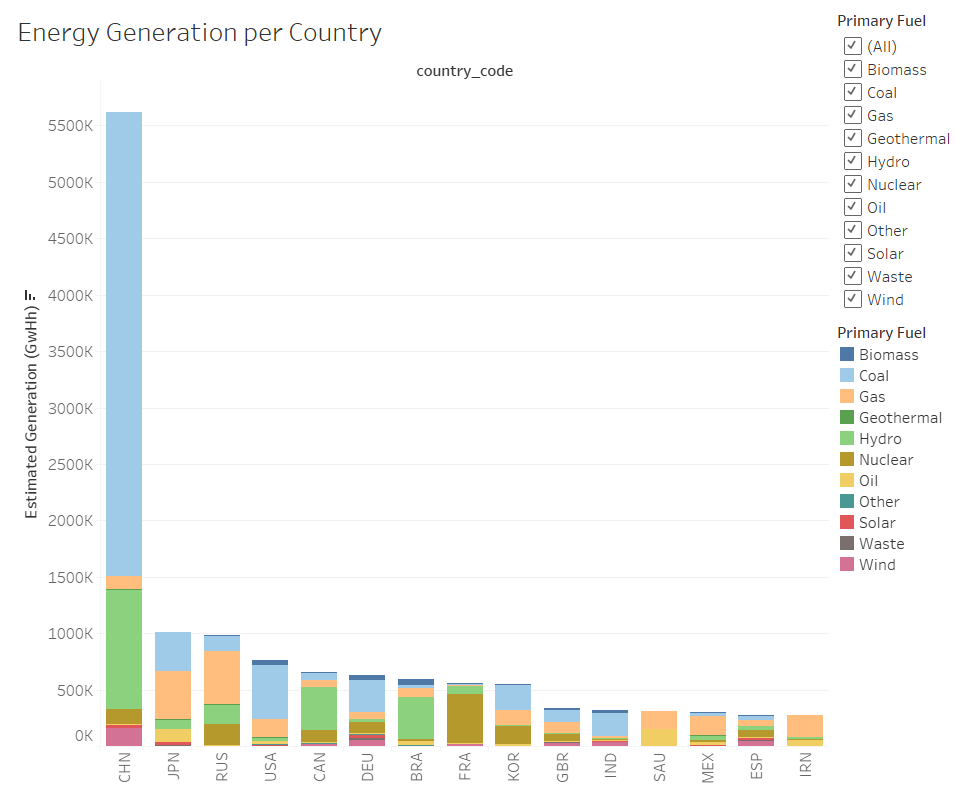
\includegraphics[scale=0.6]{Design-1.PNG}
\caption{Design 1}
\end{figure}

\begin{description}
\item[Visual Design Type:]
Stacked bar chart
\item[Name of Tool:]
Tableau
\item[Country:]
China, Japan, Russia, USA, Canada Germany, Brazil, France, South Korea, UK,  India, Saudi Arabia, Mexico, Spain, Iran
\item[Year:]
All years with data available
\item[Visual Mappings:]
\begin{itemize}
    \item[]
    \item \textbf{X axis}: Country
    \item \textbf{Y axis}: Power generation
    \item \textbf{Y axis}: Primary fuel type
\end{itemize} 
\item[Unique Observation:]
From this visualization we can see how much more energy China generates compared to the next 14 highest generating countries. We can see the breakdown of how much energy is created from the different primary fuel types within each country. For example France has a surprisingly large amount of energy generated from Nuclear power.
\item[Data Preparation:]
Data filtered to show the top 15 countries with the most power generated. Columns sorted descending by power generated. 
\end{description}

\section*{Part 1, design 2}

\begin{figure}[ht]
\centering
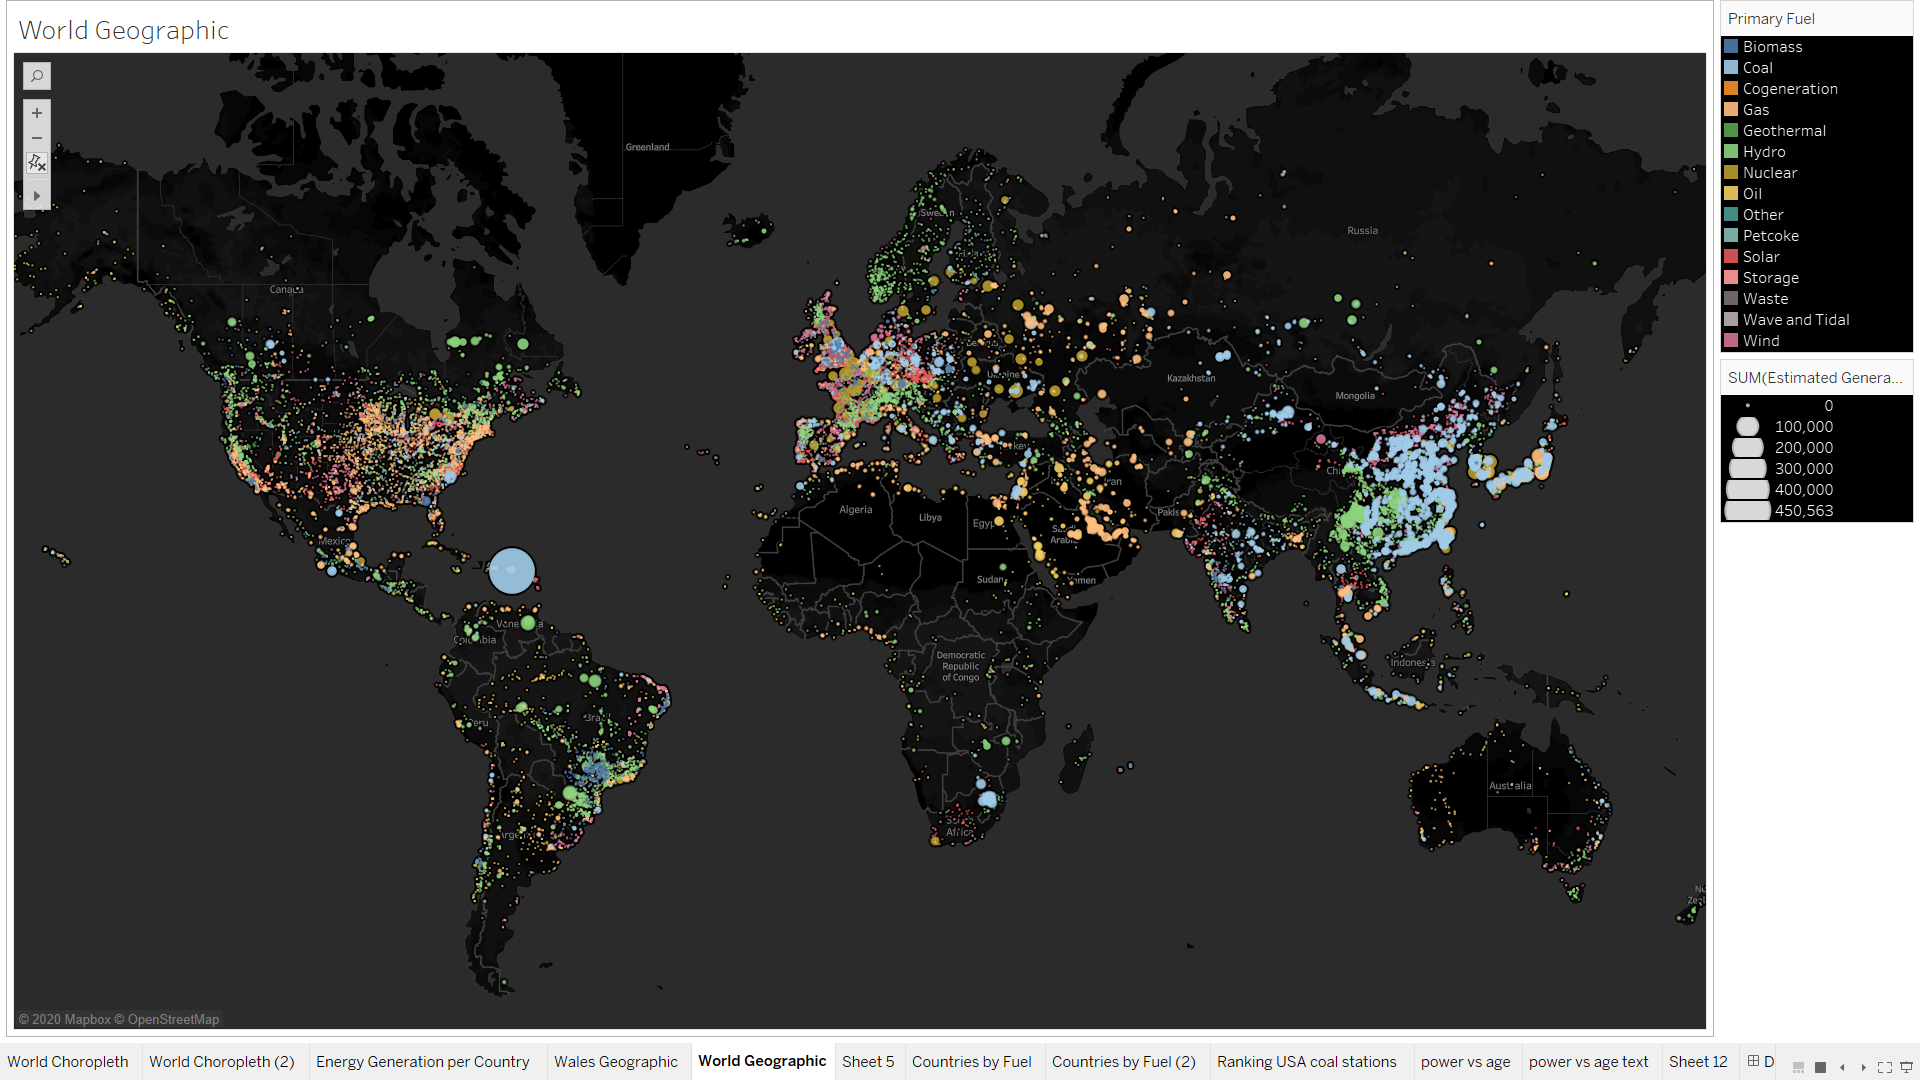
\includegraphics[scale=0.35]{Design-2.PNG}
\caption{Design 2}
\end{figure}

\begin{description}
\item[Visual Design Type:]
Symbol map
\item[Name of Tool:]
Tableau
\item[Country:]
All countries with data available
\item[Year:]
All years with data available
\item[Visual Mappings:]
\begin{itemize}
    \item[]
    \item \textbf{X axis}: Latitude
    \item \textbf{Y axis}: Longitude
    \item \textbf{Colour}: Primary fuel type
\end{itemize} 
\item[Unique Observation:]
From this visualization we can see how the location of power plants seem to correlate with the population centres of the world such as Western Europe and Southeast Asia.
There is a station that appears to produce much more power than any other station in the world located in Puerto Rico.
It is a coal station and produced 450,000 GWh.
\item[Data Preparation:]
Data filtered to remove stations if they had no available data or 0 for the  estimated generation field to reduce clutter.
\end{description}


\section*{Part 1, design 3}

\begin{figure}[ht]
\centering
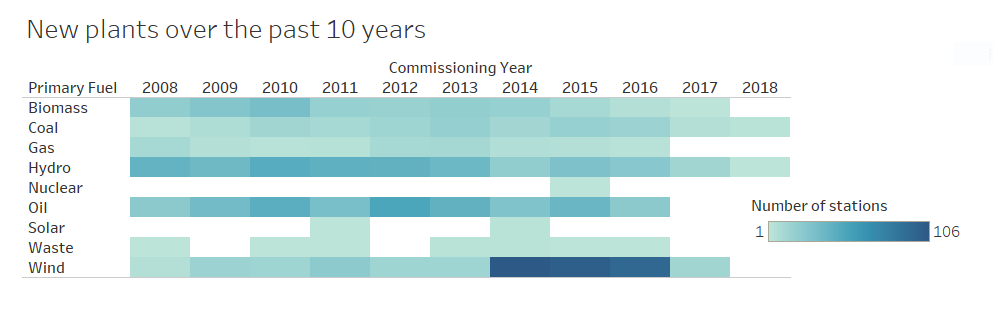
\includegraphics[scale=0.6]{NewPlants.PNG}
\caption{Design 3}
\end{figure}

\begin{description}
\item[Visual Design Type:]
Temporal heatmap
\item[Name of Tool:]
Tableau
\item[Country:]
All countries with data available
\item[Year:]
Years between 2008 and 2018, inclusive
\item[Visual Mappings:]
\begin{itemize}
    \item[]
    \item \textbf{X axis}: Commission year
    \item \textbf{Y axis}: Primary fuel type
    \item \textbf{Colour}: Number of stations
\end{itemize} 
\item[Unique Observation:]
This visualisation shows the recent power plant commission trends.
Nuclear and solar plants have not been popular over the past 10 years.
Alternatively many wind plants have opened, particularly in the 2014 to to 2016 period.
\item[Data Preparation:]
 Commission year filtered to show records between 2008 and 2018, inclusive. 
 Many records had no commission data for generation were removed.
\end{description}


\section*{Part 1, design 4}

\begin{figure}[ht]
\centering
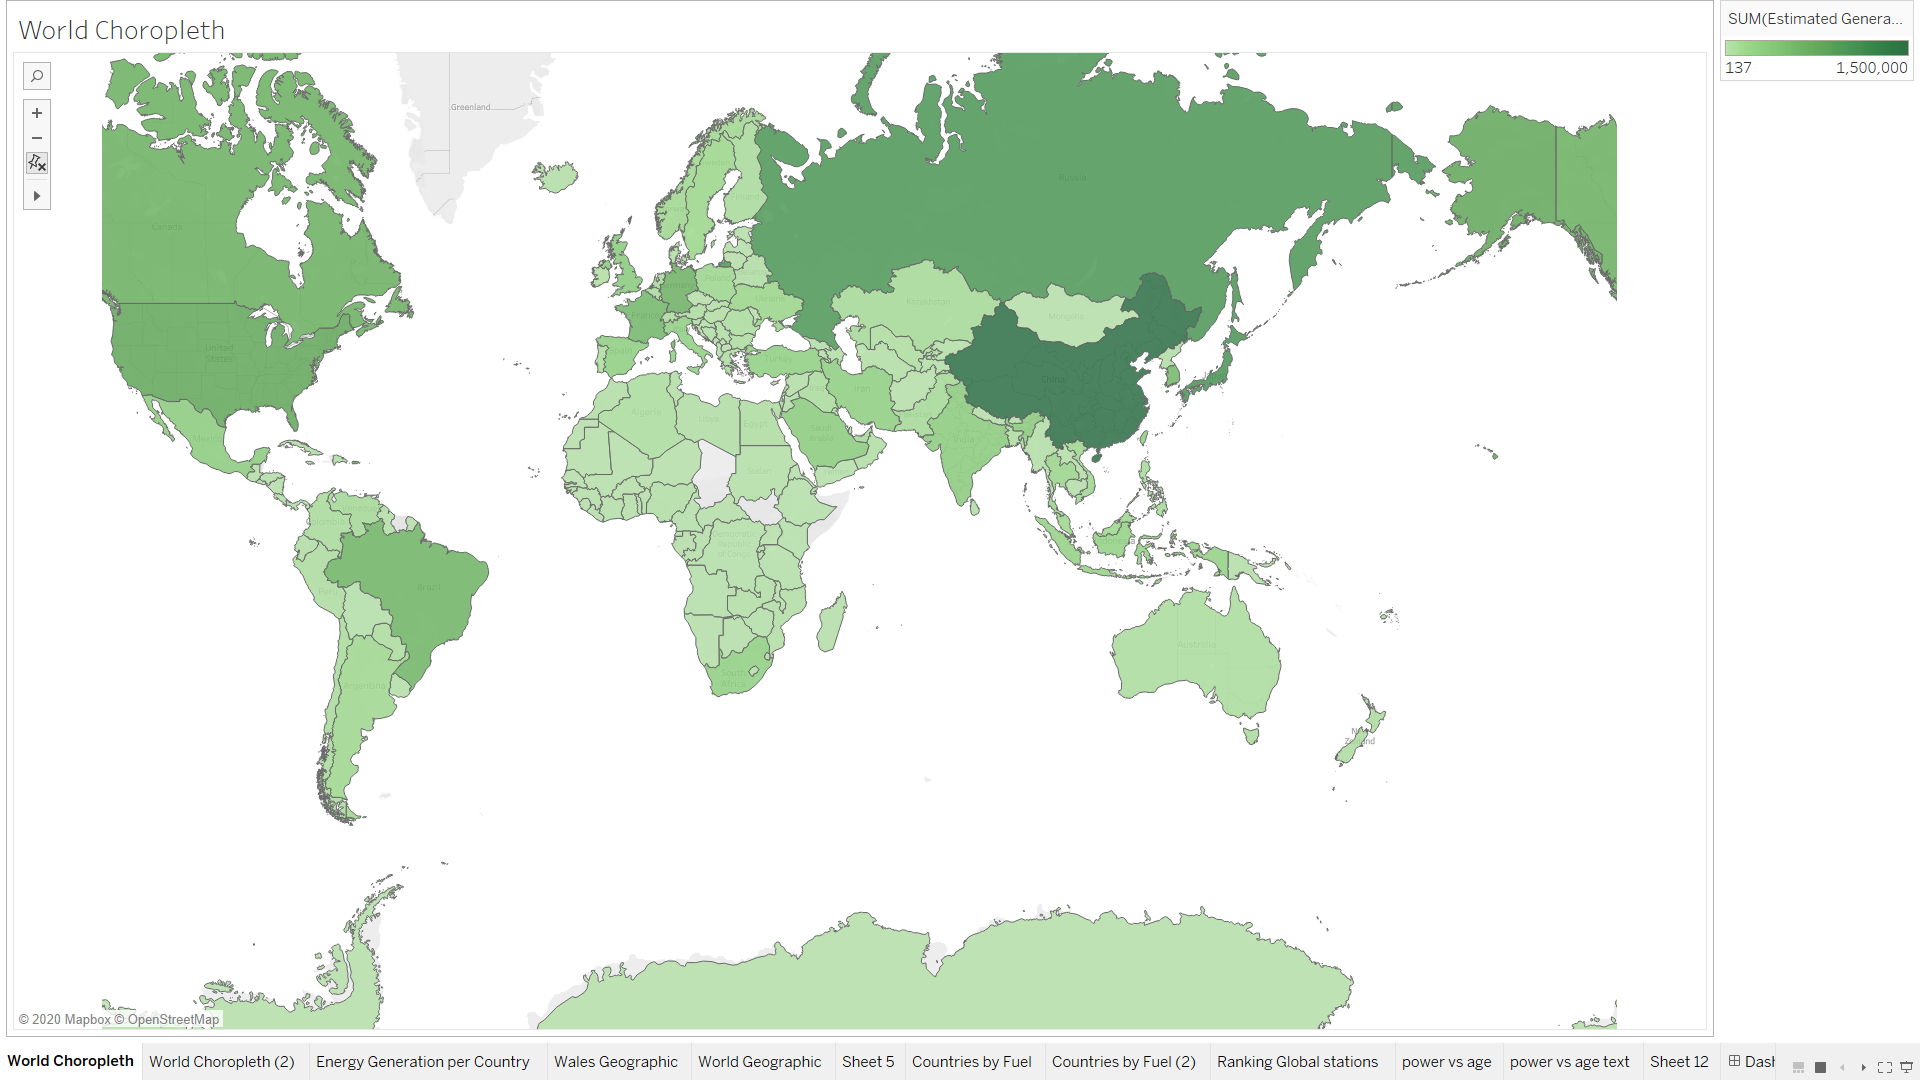
\includegraphics[scale=0.3]{World-Choropleth.PNG}
\caption{Design 4}
\end{figure}

\begin{description}
\item[Visual Design Type:]
Choropleth
\item[Name of Tool:]
Tableau
\item[Country:]
All countries with available data
\item[Year:]
All years with data available
\item[Visual Mappings:]
\begin{itemize}
    \item[]
    \item \textbf{X axis}: Latitude
    \item \textbf{Y axis}: Longitude
    \item \textbf{Colour}: Power generation 
    
\end{itemize} 
\item[Unique Observation:]
China generates much more power than any other country. 
South America and Africa produce less power than the other continents.
\item[Data Preparation:]
Colour map starts at 0 and stops at 1,500,000. 
This the colour mappings are spread between these values and any higher values will be shown as 1,500,000.

\end{description}


\section*{Part 1, design 5}

\begin{figure}[ht]
\centering
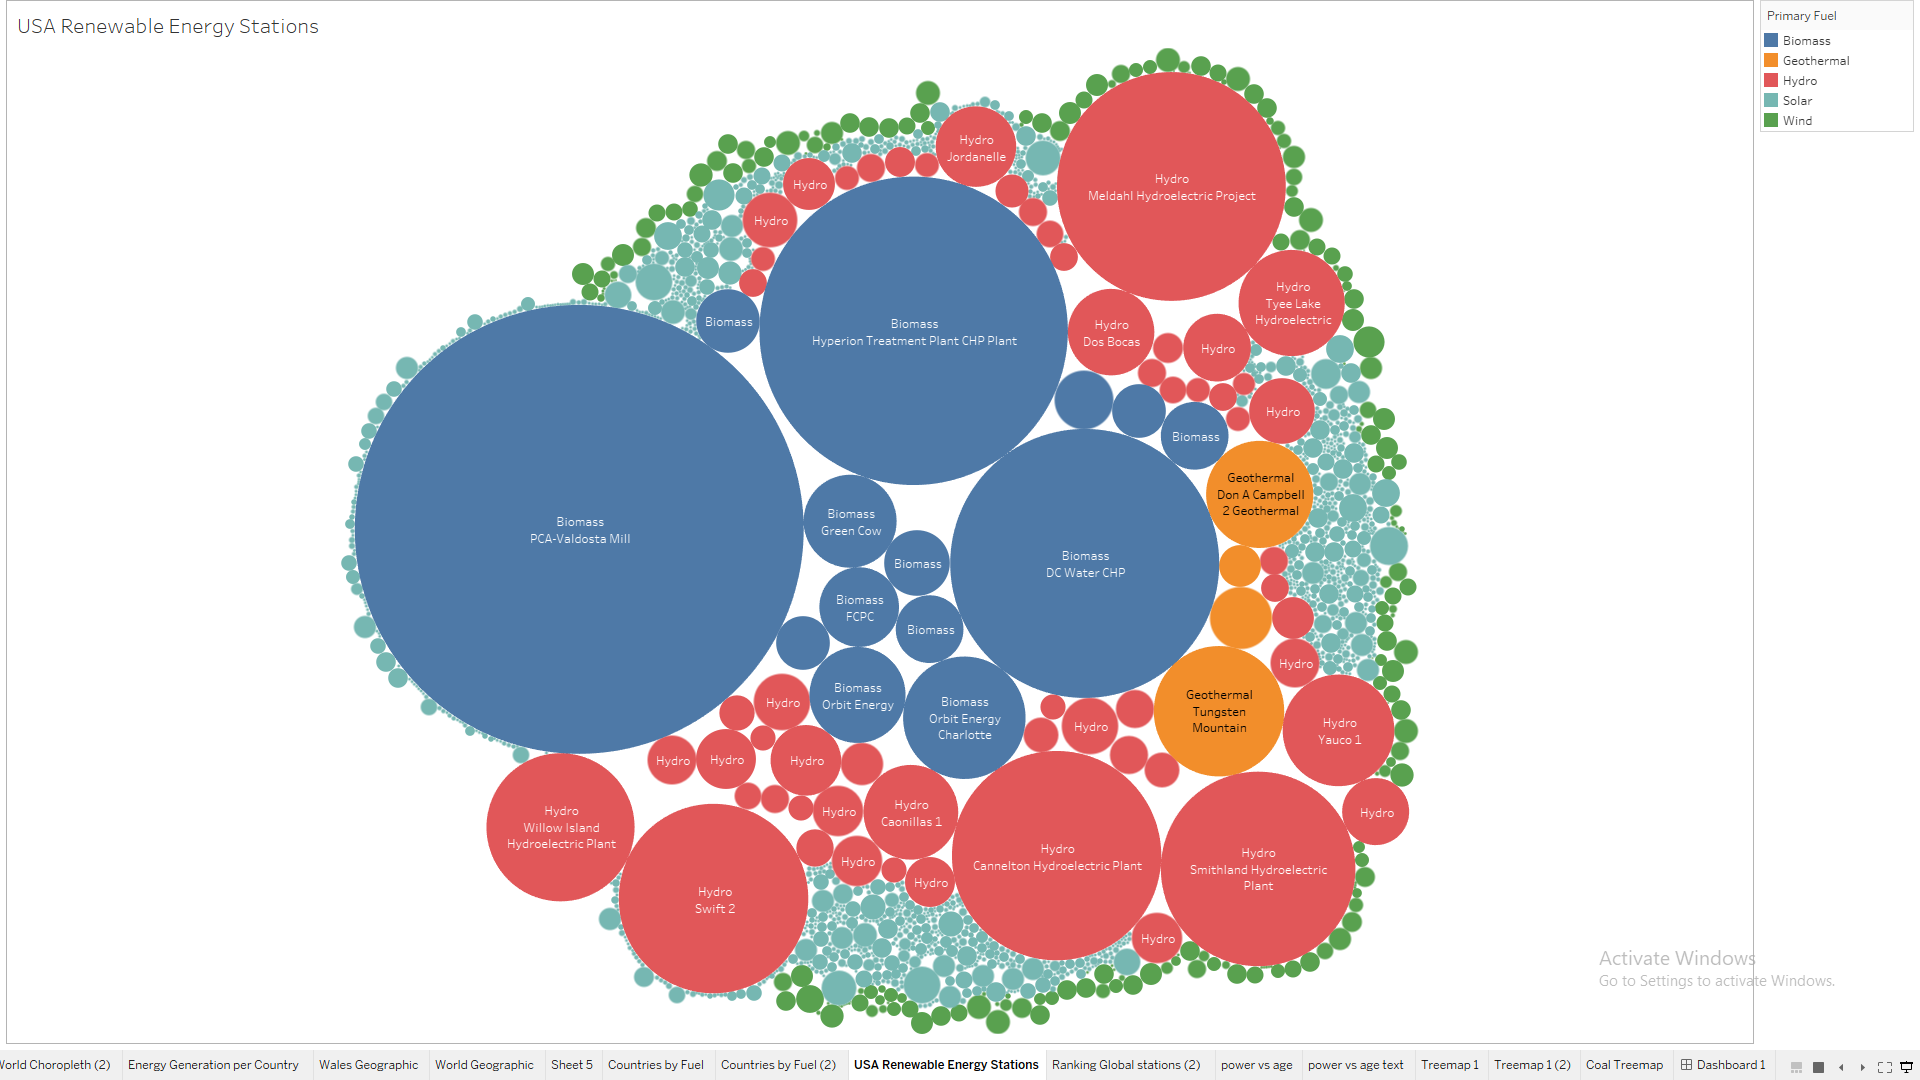
\includegraphics[scale=0.3]{Packed-Bubbles.PNG}
\caption{Design 3}
\end{figure}

\begin{description}
\item[Visual Design Type:]
Packed bubbles
\item[Name of Tool:]
Tableau
\item[Country:]
USA
\item[Year:]
All years with data available
\item[Visual Mappings:]
\begin{itemize}
    \item[]
    \item \textbf{Colour}: Primary fuel type
    \item \textbf{Size}: Power generation
\end{itemize} 
\item[Unique Observation:]
This visualisation shows that while the USA has a small number of coal plants compared to solar, and wind, those stations produce much more power per plant.
We can see how solar and wind plants produce only a small amount of energy each so many are needed to produce meaningful amounts of energy.

\item[Data Preparation:]
Data filtered to show only USA stations. 
Stations with 0 or no data for generation were removed.
\end{description}


\section*{Part 2}

\begin{figure}[ht]
\centering
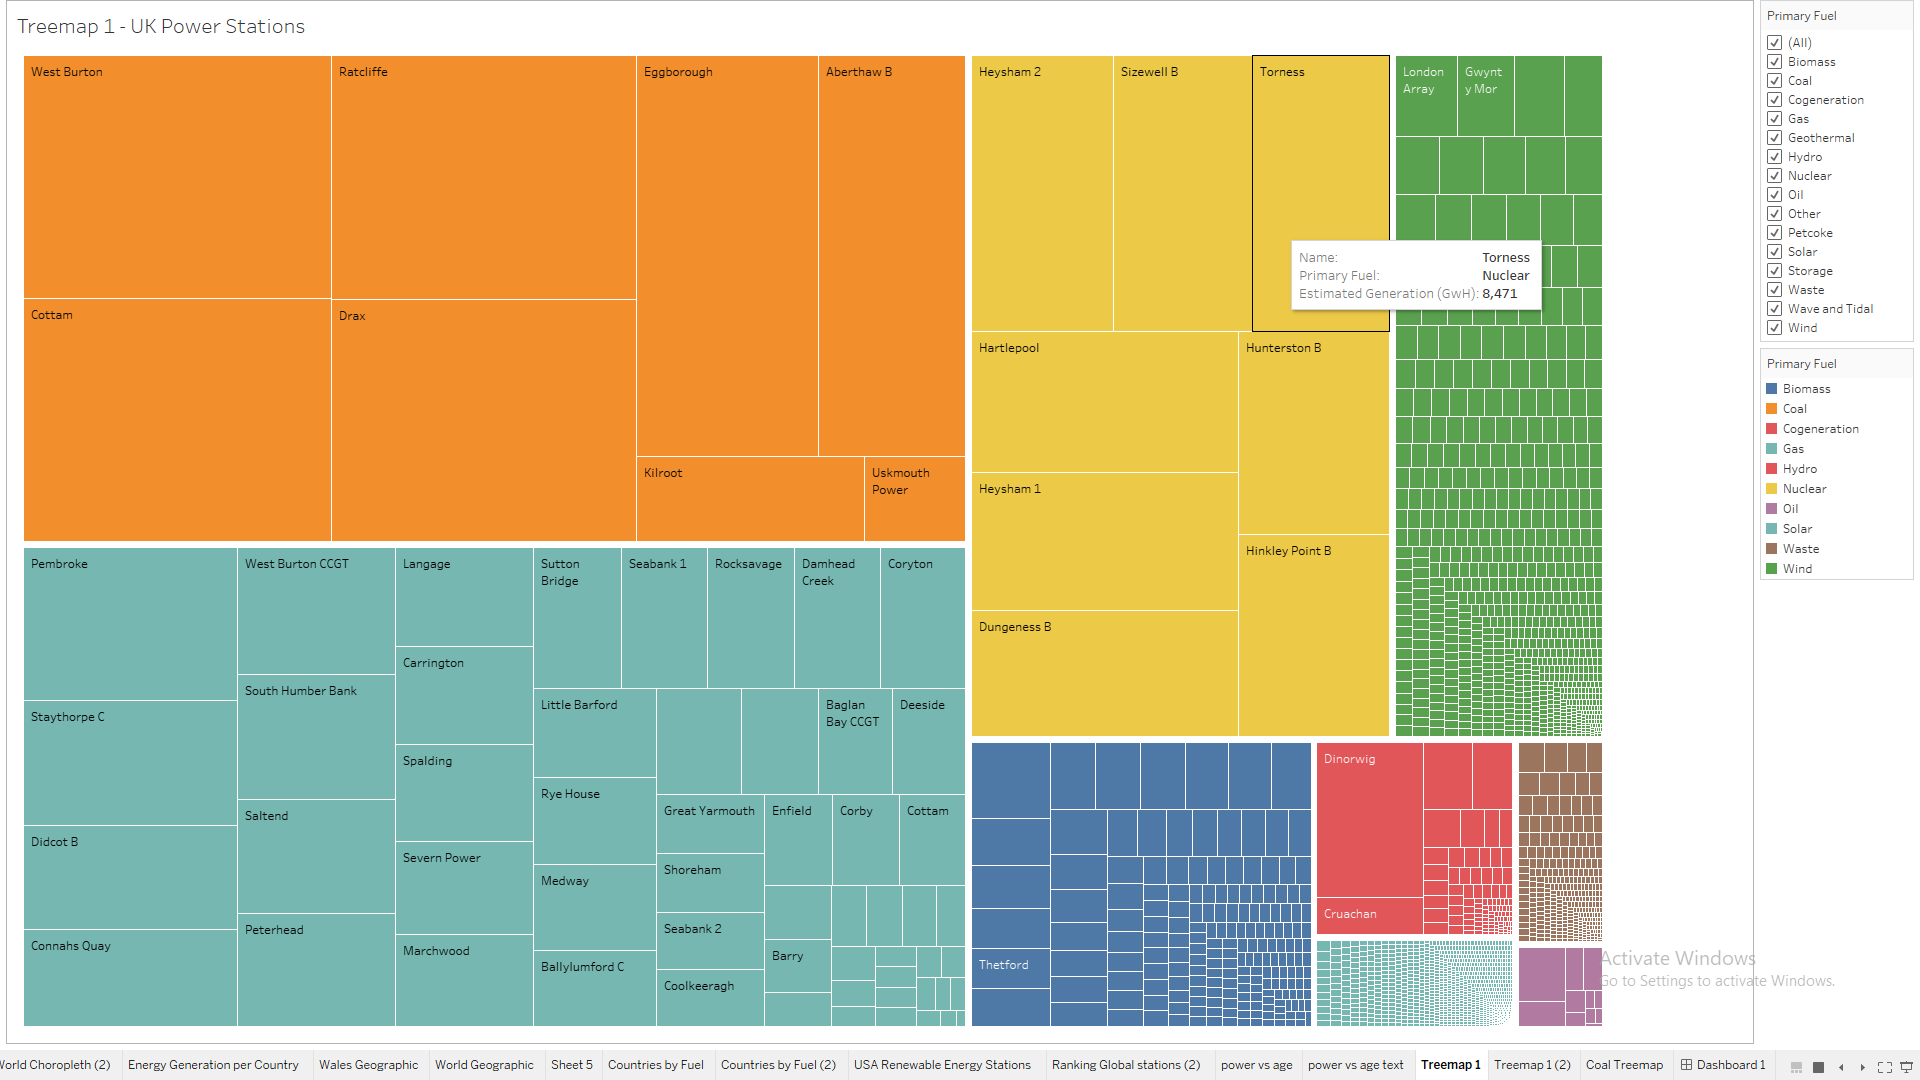
\includegraphics[scale=0.3]{Treemap.PNG}
\caption{A treemap}
\end{figure}

\begin{description}
\item[Name of Tool:]
Tableau
\item[Country:]
UK
\item[Year:]
All years with data available
\item[Data Preparation:]
Data filtered to show UK stations only.
\item[Colour:]
Primary fuel type
\item[Tooltip:]
Station name, Primary fuel type, power generation


\item[Hierarchy:]

\begin{itemize}
    \item[]
    \item The data hierarchy shown in the treemap is the subdivision of the UK's total power generation between the different primary fuel types, and the individual plants within each fuel type.
    \item Leaf node size is mapped to power generation of an individual power station.
    \item Leaf nodes are ordered from highest power generation to lowest.
    \item Internal nodes are mapped to categories of primary fuel type.
    \item Internal node size is mapped to the total power generation of a primary fuel type. 
    \item The squarified algorithm has been used to create the treemap. 
\end{itemize} 
\end{description}

\section*{Part 3}

\begin{figure}[ht]
\centering
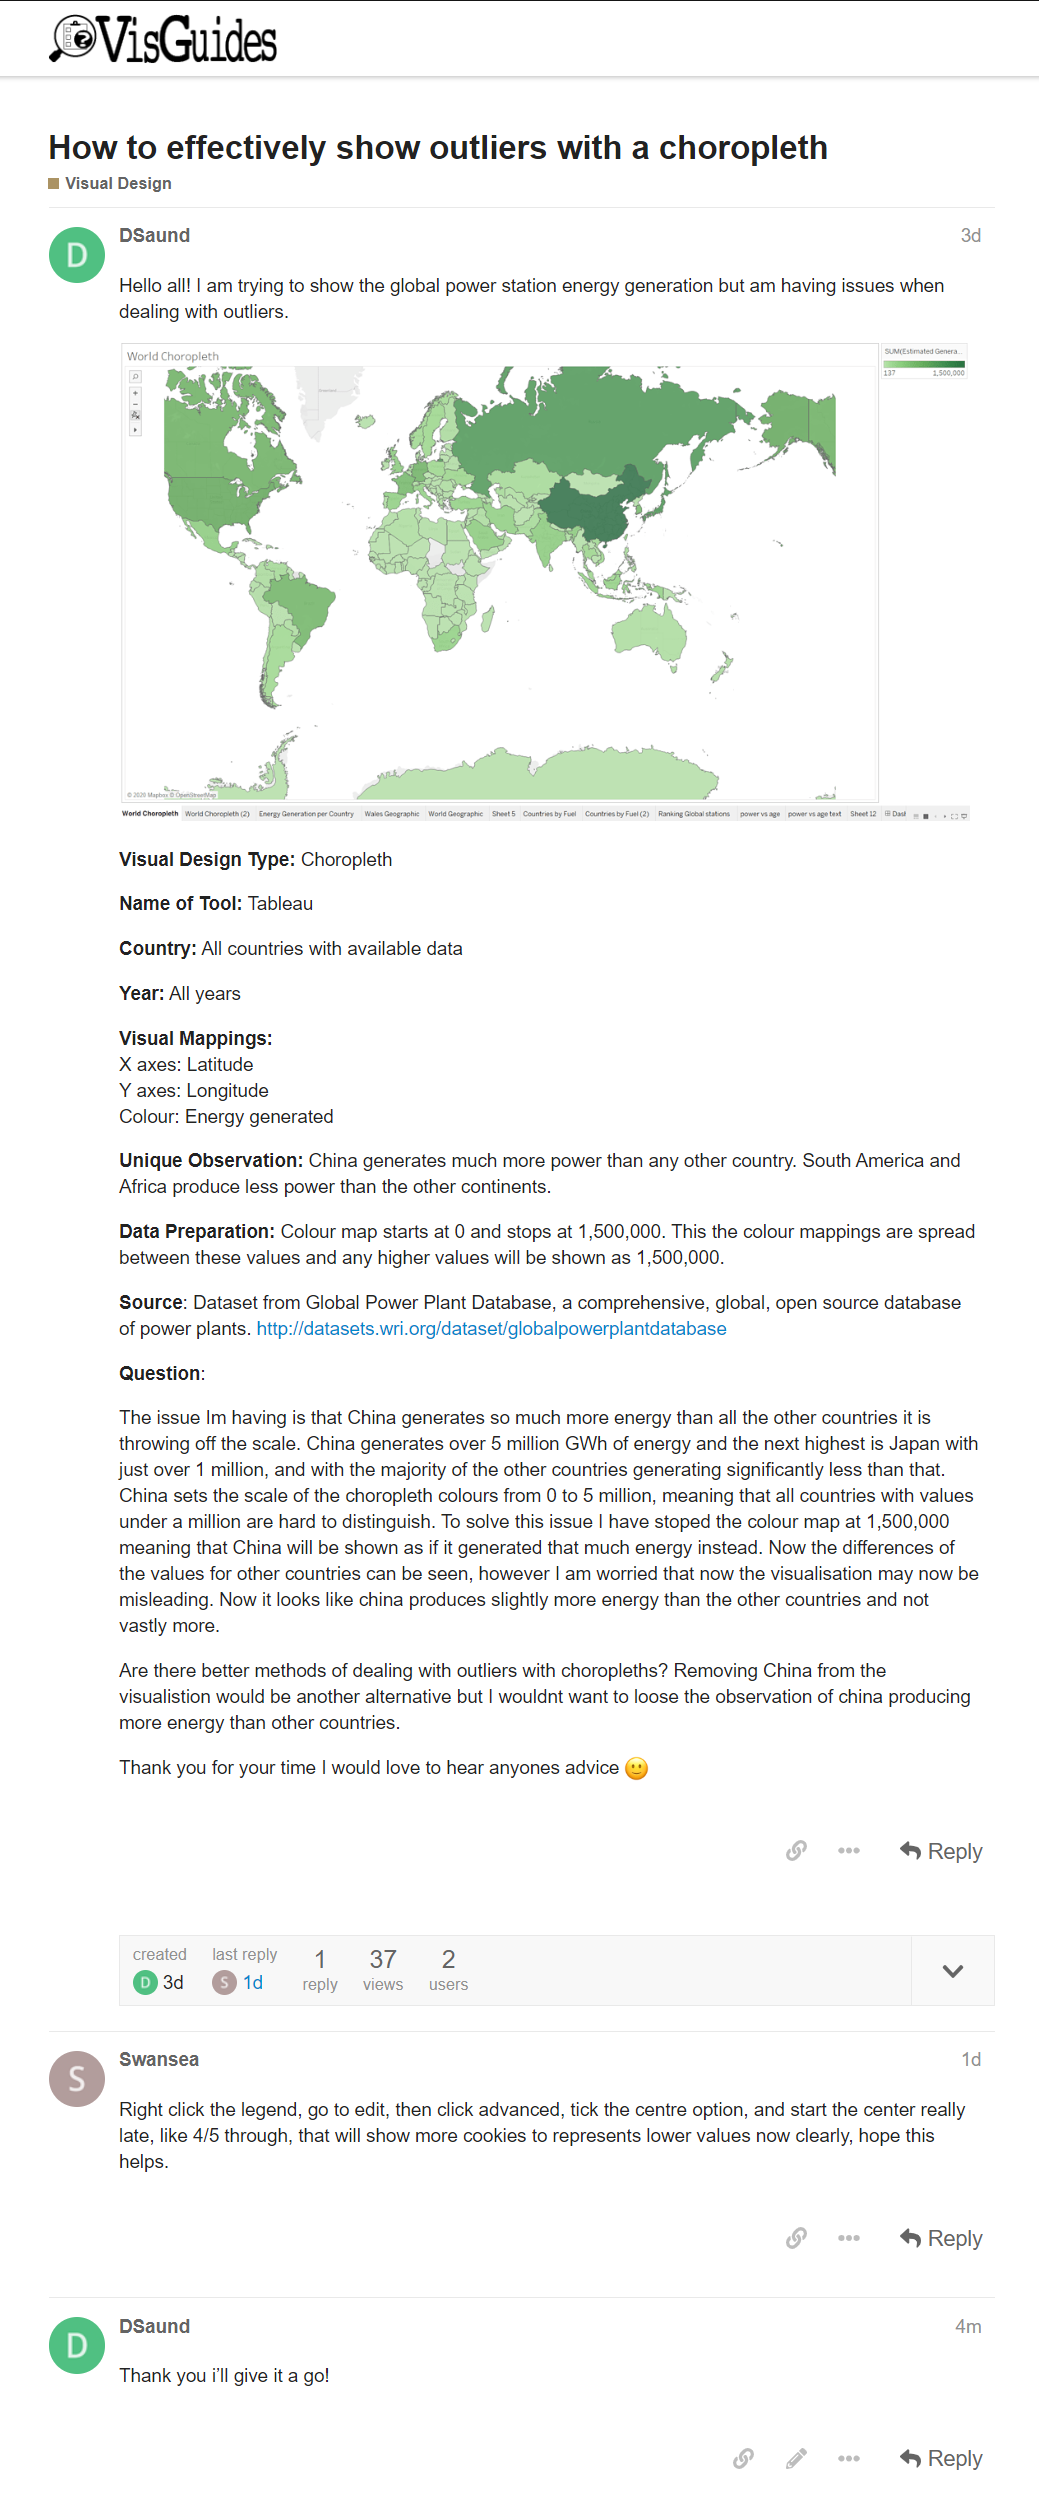
\includegraphics[scale=0.25]{VisGuides.png}
\caption{VisGuides screenshot}
\end{figure}

\end{document}
